\section{Context}
Technologies have revolutionised the manufacturing industry ever since the Industrial revolution in the 19th century.
Robots are increasing productivity by replacing humans for arduous and repetitive manual tasks.
%are increasing productivity, efficiency, lower costs, and relieve humans from operationally dangerous tasks.
Increasing order requests for industrial robots has led to higher capital investments into the field.
Although robots can be superior in automating human tasks, there remain many that cannot be completely taken over and still need human intervention (\eg high-precision tasks).
To allow both human precision and robot automation, collaborative robots have been introduced.

\subsection{Cobotics}\label{subsec:Cobotics}
Collaborative robots, or \textit{cobots}, have been introduced by \cite{colgate1999cobots} and allow for a close collaboration between humans and robots.
They enable humans to perform tasks that they cannot perform on their own, due to physical constraints such as the manipulation of heavy parts.
Furthermore, they reduce risks of work-related accidents, including health hazards such as exposure to dangerous environments (\eg chemical acids, excessive temperatures or noise), as well as sleeping disorders caused by rotating work shifts.
Cobots contribute to productivity gains as they are designed to take over manual and repetitive tasks while responding to actions of the human operator.
While replacing jobs of low-skilled human workers, they open up a market for new high-skilled jobs.

Cobotic systems have been adopted in several industries from the food-processing industry (\cite{Food}), to aeronautics (\cite{Airbus}), to the health industry (\cite{Ebola}).
However, companies resist the use of robots in their daily routines as they consider the investment cost ineffective, due to their high initial costs and the lack of trained personnel.
%, who have the needed programming skills to fully operate and exploit the robots.
Traditional robot programming solutions require domain experts and robots are generally programmed to complete a specific task.
Recent approaches using large amounts of data (\eg Neural Networks (\cite{billard2001robust})) or self-exploration (\eg Reinforcement Learning (\cite{smart2002effective})) become infeasible for task-specific applications.
This is a bottleneck for industries and many robot programming solutions fail as the deployment in real-world scenarios introduces further limitations. 
Thus, recent research has been focusing on robot programming for end-users, in particular Robot Programming by Demonstration.

\subsection{Robot Programming by Demonstration}
Robot Programming by Demonstration (PbD), also referred to as \textit{Learning from Demonstration}, is an end-user programming technique for teaching a robot new skills by demonstrating a task, without writing code (\cite{billard2008robot}).
Influenced by natural learning paradigms in humans and other animals, it is an intuitive robot programming method, with the goal to refine the robot's performance, by providing repetitive demonstrations.
PbD has become a central topic in research areas, with the aim to move from purely pre-programmed robots to flexible user-based interfaces for training robots.

Figure \ref{fig:Principle Overview} shows the life-cycle for teaching a robot by demonstration that consists of three main steps.
The teacher demonstrates a new skill to the robot.
The robot uses its sensors for a multi-modal perception of the demonstration and extracts the relevant information to create a model of the skill.
The skill is applied in a new context and the execution is evaluated by the teacher.
The teacher can refine the taught skill by providing additional demonstrations.
The robot then generalises over the demonstrations by extracting relevant features. %that remained unchanged across the set of demonstrations.
This incremental learning process allows non-robotics users to teach the robot new skills by providing demonstrations.

\begin{figure}[h]
	\centering
	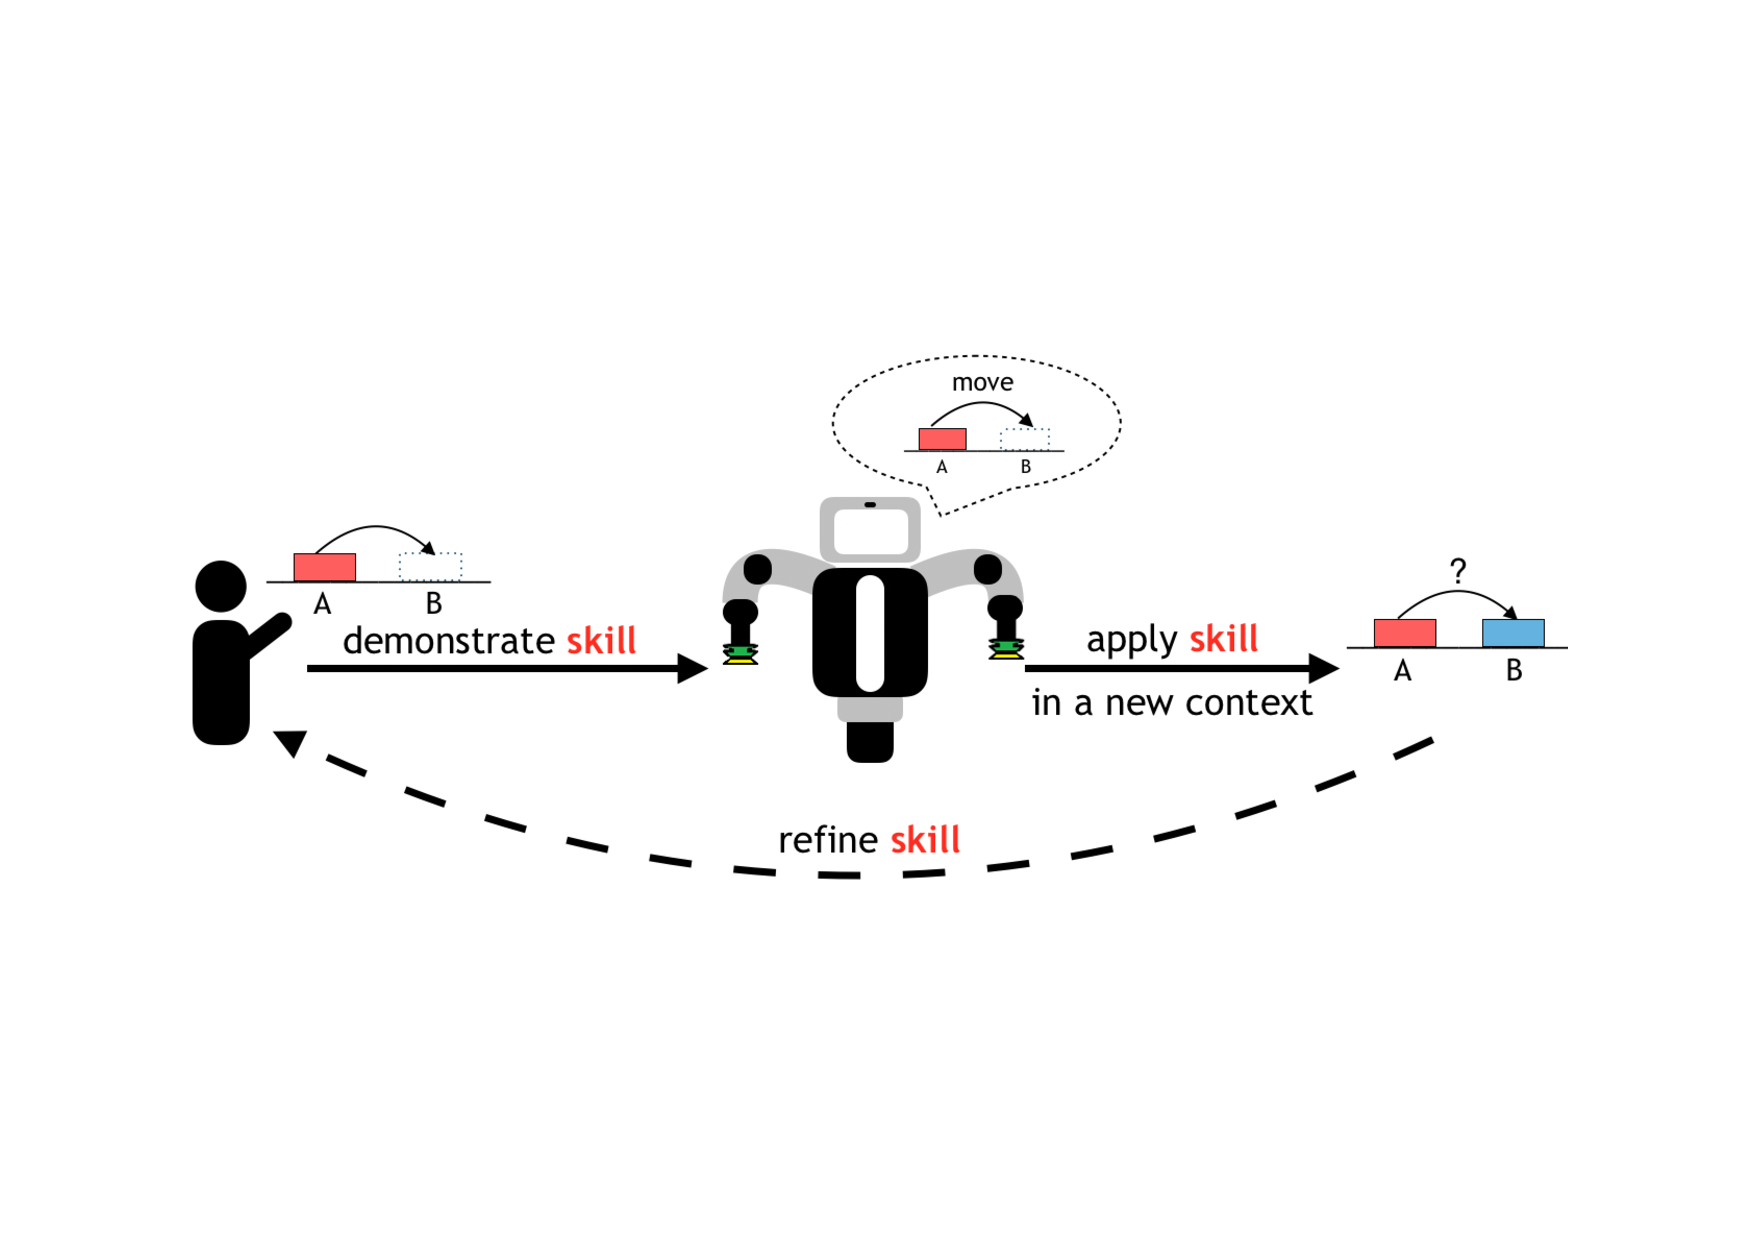
\includegraphics[width=0.75\linewidth]{figures/PbD-Overview}
	\caption{Overview of the Programming by Demonstration life-cycle consisting of three steps}
	\label{fig:Principle Overview}
\end{figure}

%Besides the advantage of being able to teach the robot tasks without the need to write code, PbD provides a powerful tool to improve learning abilities by reducing the search space of possible solutions.
However, as the robot has limited knowledge about the world and restricted sensor availability, learning object manipulation tasks is still considered a hard problem (\cite{ekvall2008robot}).
Many PbD algorithms have been proposed in the literature (\cite{argall2009survey,billing2010formalism}), but there still remain several challenges, such as the suboptimality of demonstrations (\cite{chen2003programing,kaiser1995obtaining}) or the lack of comparative user studies (\cite{suay2012practical}).
% teaching full action sequences
Another major problem is that the robot is generally demonstrated an action sequence to complete a specific task (\cite{orendt2016robot,peppoloni2014ros}), rather than individual reusable actions.
Take for example the Tower of Hanoi problem (\cite{douglas1985metamagical}) as shown in \fig{fig:Tower of Hanoi 3}.
The objective is to move the entire stack from one peg to another, while obeying the following rules:
\begin{itemize}
\item Only one disk can be moved at a time,
\item each move consists of taking the upper disk from one of the stacks and placing it on top of another (possibly empty) stack, and
\item no disk may be placed on top of a smaller disk.
\end{itemize}

The robot can be taught an action sequence to solve the problem for three disks.
When the problem changes to four disks (\fig{fig:Tower of Hanoi 4}, the robot has to be demonstrated a new sequence, even though both problems obey the same rules.
This reprogramming process can be complicated and time-consuming as it does not allow to generalise for different tasks.
A more efficient approach would be to teach the robot the primitive action of moving a disk, associate rules or \textit{conditions} to this action (\eg disks can only be placed on top of larger ones), and have the robot generate an optimal solution automatically, for example using an automated planner.

\begin{figure}[htp]
	\centering
	\begin{subfigure}[t]{0.45\textwidth}
		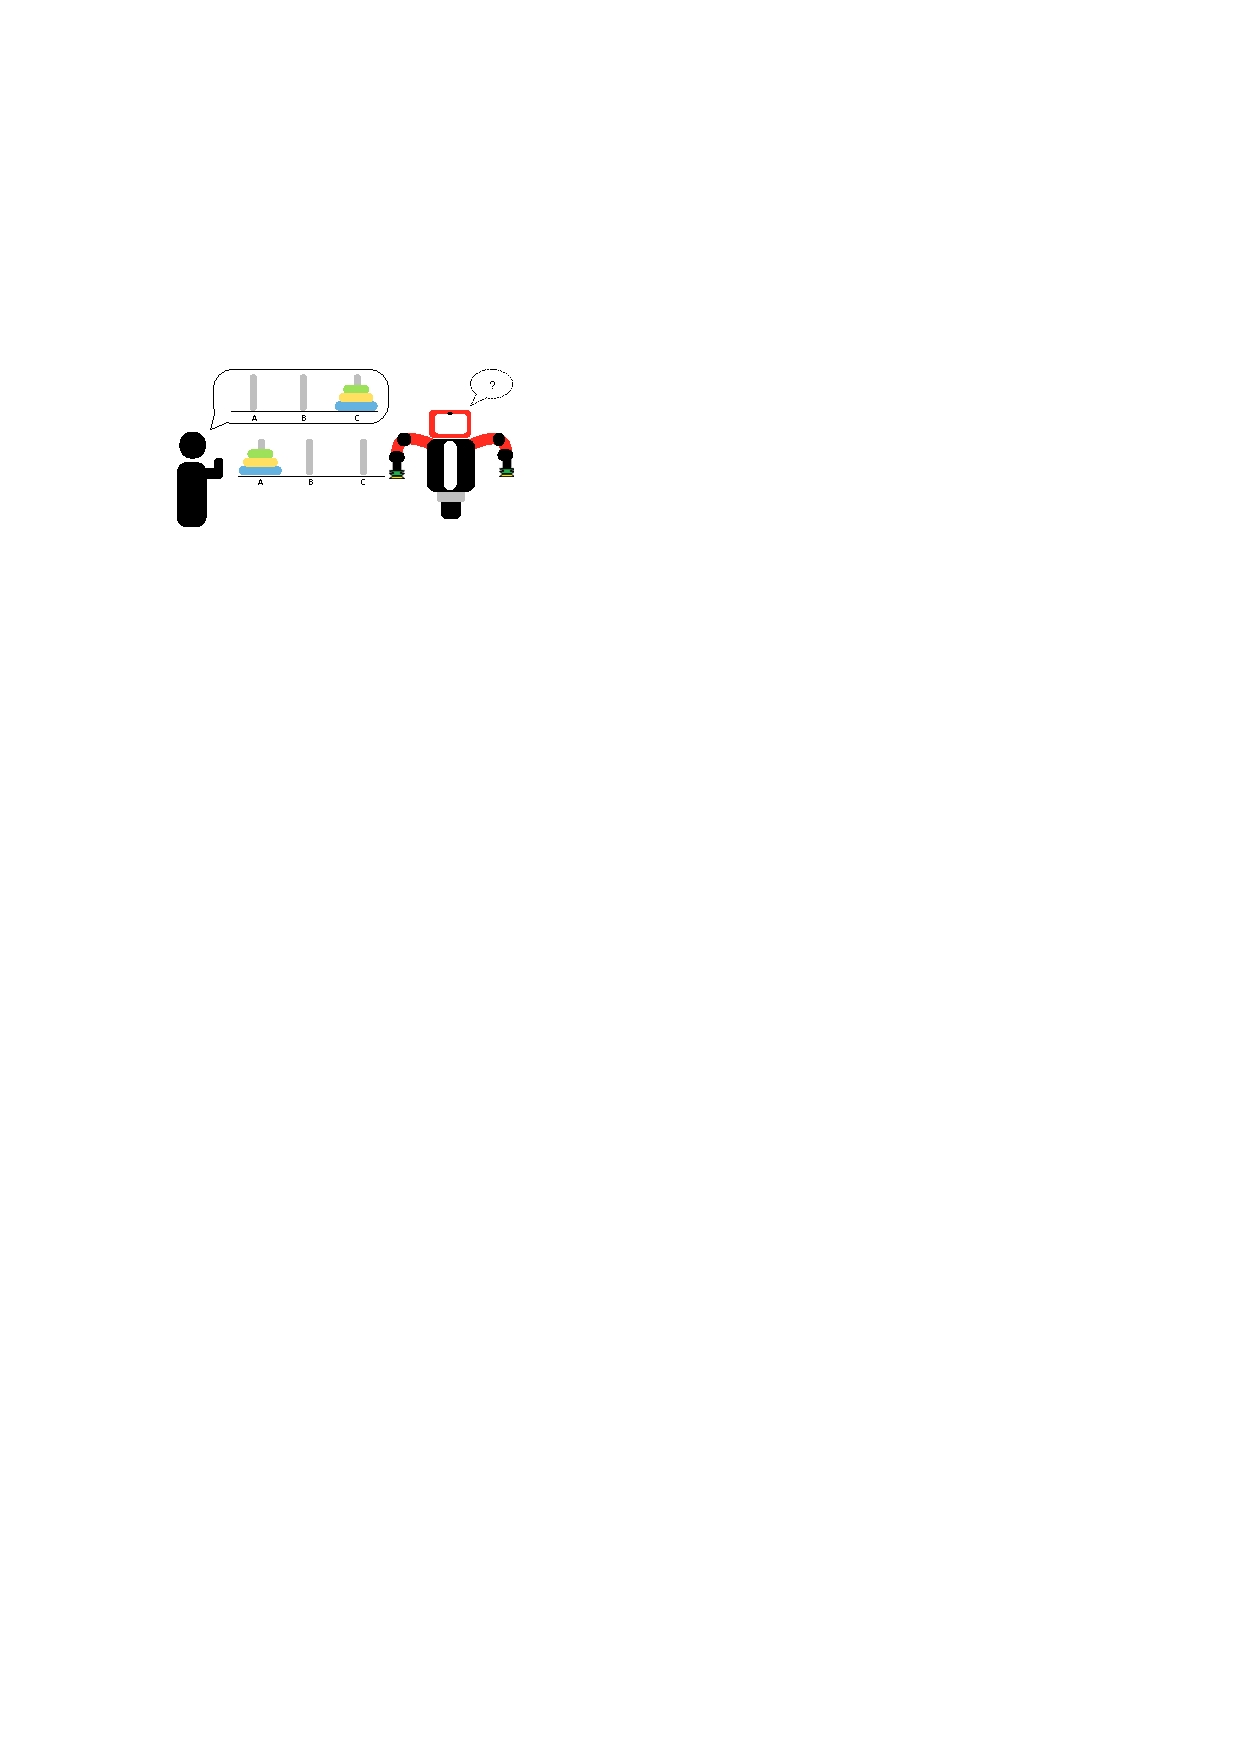
\includegraphics[width=\textwidth]{figures/hanoi-0}
		\caption{with three disks}		
		\label{fig:Tower of Hanoi 3}
	\end{subfigure}\hfill
\begin{subfigure}[t]{0.45\textwidth}
	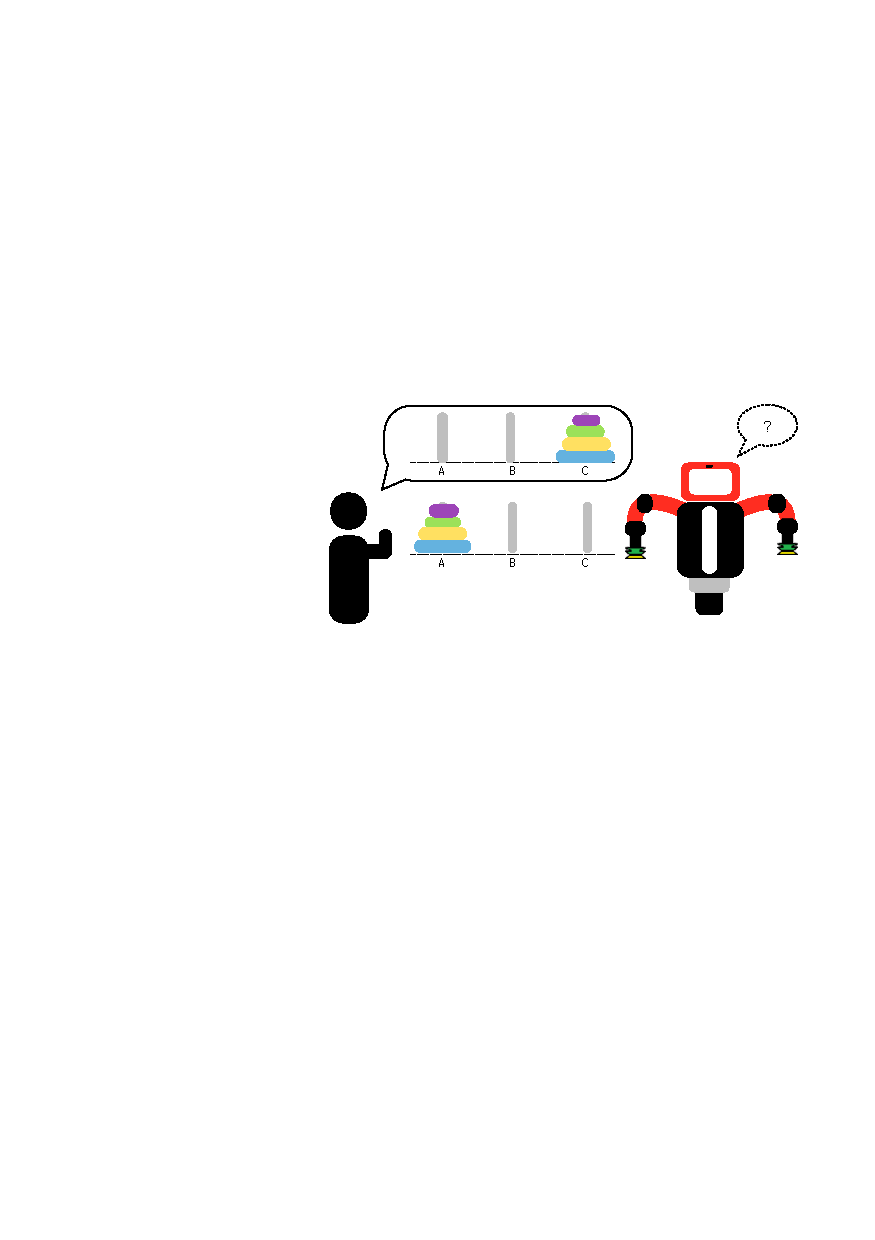
\includegraphics[width=\textwidth]{figures/hanoi-1}
	\caption{with four disks}
	\label{fig:Tower of Hanoi 4}
\end{subfigure}
	
	\caption{Tower of Hanoi problem where the goal is to move the entire stack of disks from one peg to another}
	\label{fig:Tower of Hanoi}
\end{figure}

\subsection{Automated Planning}
Automated Planning, also known as \textit{AI Planning}, is a research field that focuses on the development of efficient search algorithms to generate solutions to problems (\cite{ghallab2004automated}).
Given a set of actions, a description of the state of the world, and some goal state, the planner generates a sequence of actions, which guarantees the transition from the initial state to the goal state (\fig{fig:Planning domain}).
To allow a correct transition between different world states, actions are defined in terms of preconditions and effects, which represent states before and after the action execution respectively (\fig{fig:Planning action}).
Planning algorithms use a symbolic planning language such as STRIPS (\cite{fikes1971strips}) or PDDL (\cite{ghallab2004automated}) as their standard encoding language.
The Tower of Hanoi problem could be defined in terms of a planning problem, where the domain consists of 3 pegs and a number of disks, and the action is defined as moving a disk from one peg to another.
A planner can then be used to generate a solution for any number of disks.
%In the initial state, the disks are stacked in ascending order (smallest at the top) on one of the pegs, in the goal state the disks are stacked in the same order on one of the other two remaining pegs. 
%The goal state must be achieved by obeying certain rules for moving the disks (\eg only the top disk of a stack can be moved at a time and may not be placed on top of a smaller disk). 


\begin{figure}[htp]
	\centering
	
	\begin{subfigure}[t]{0.54\textwidth}
		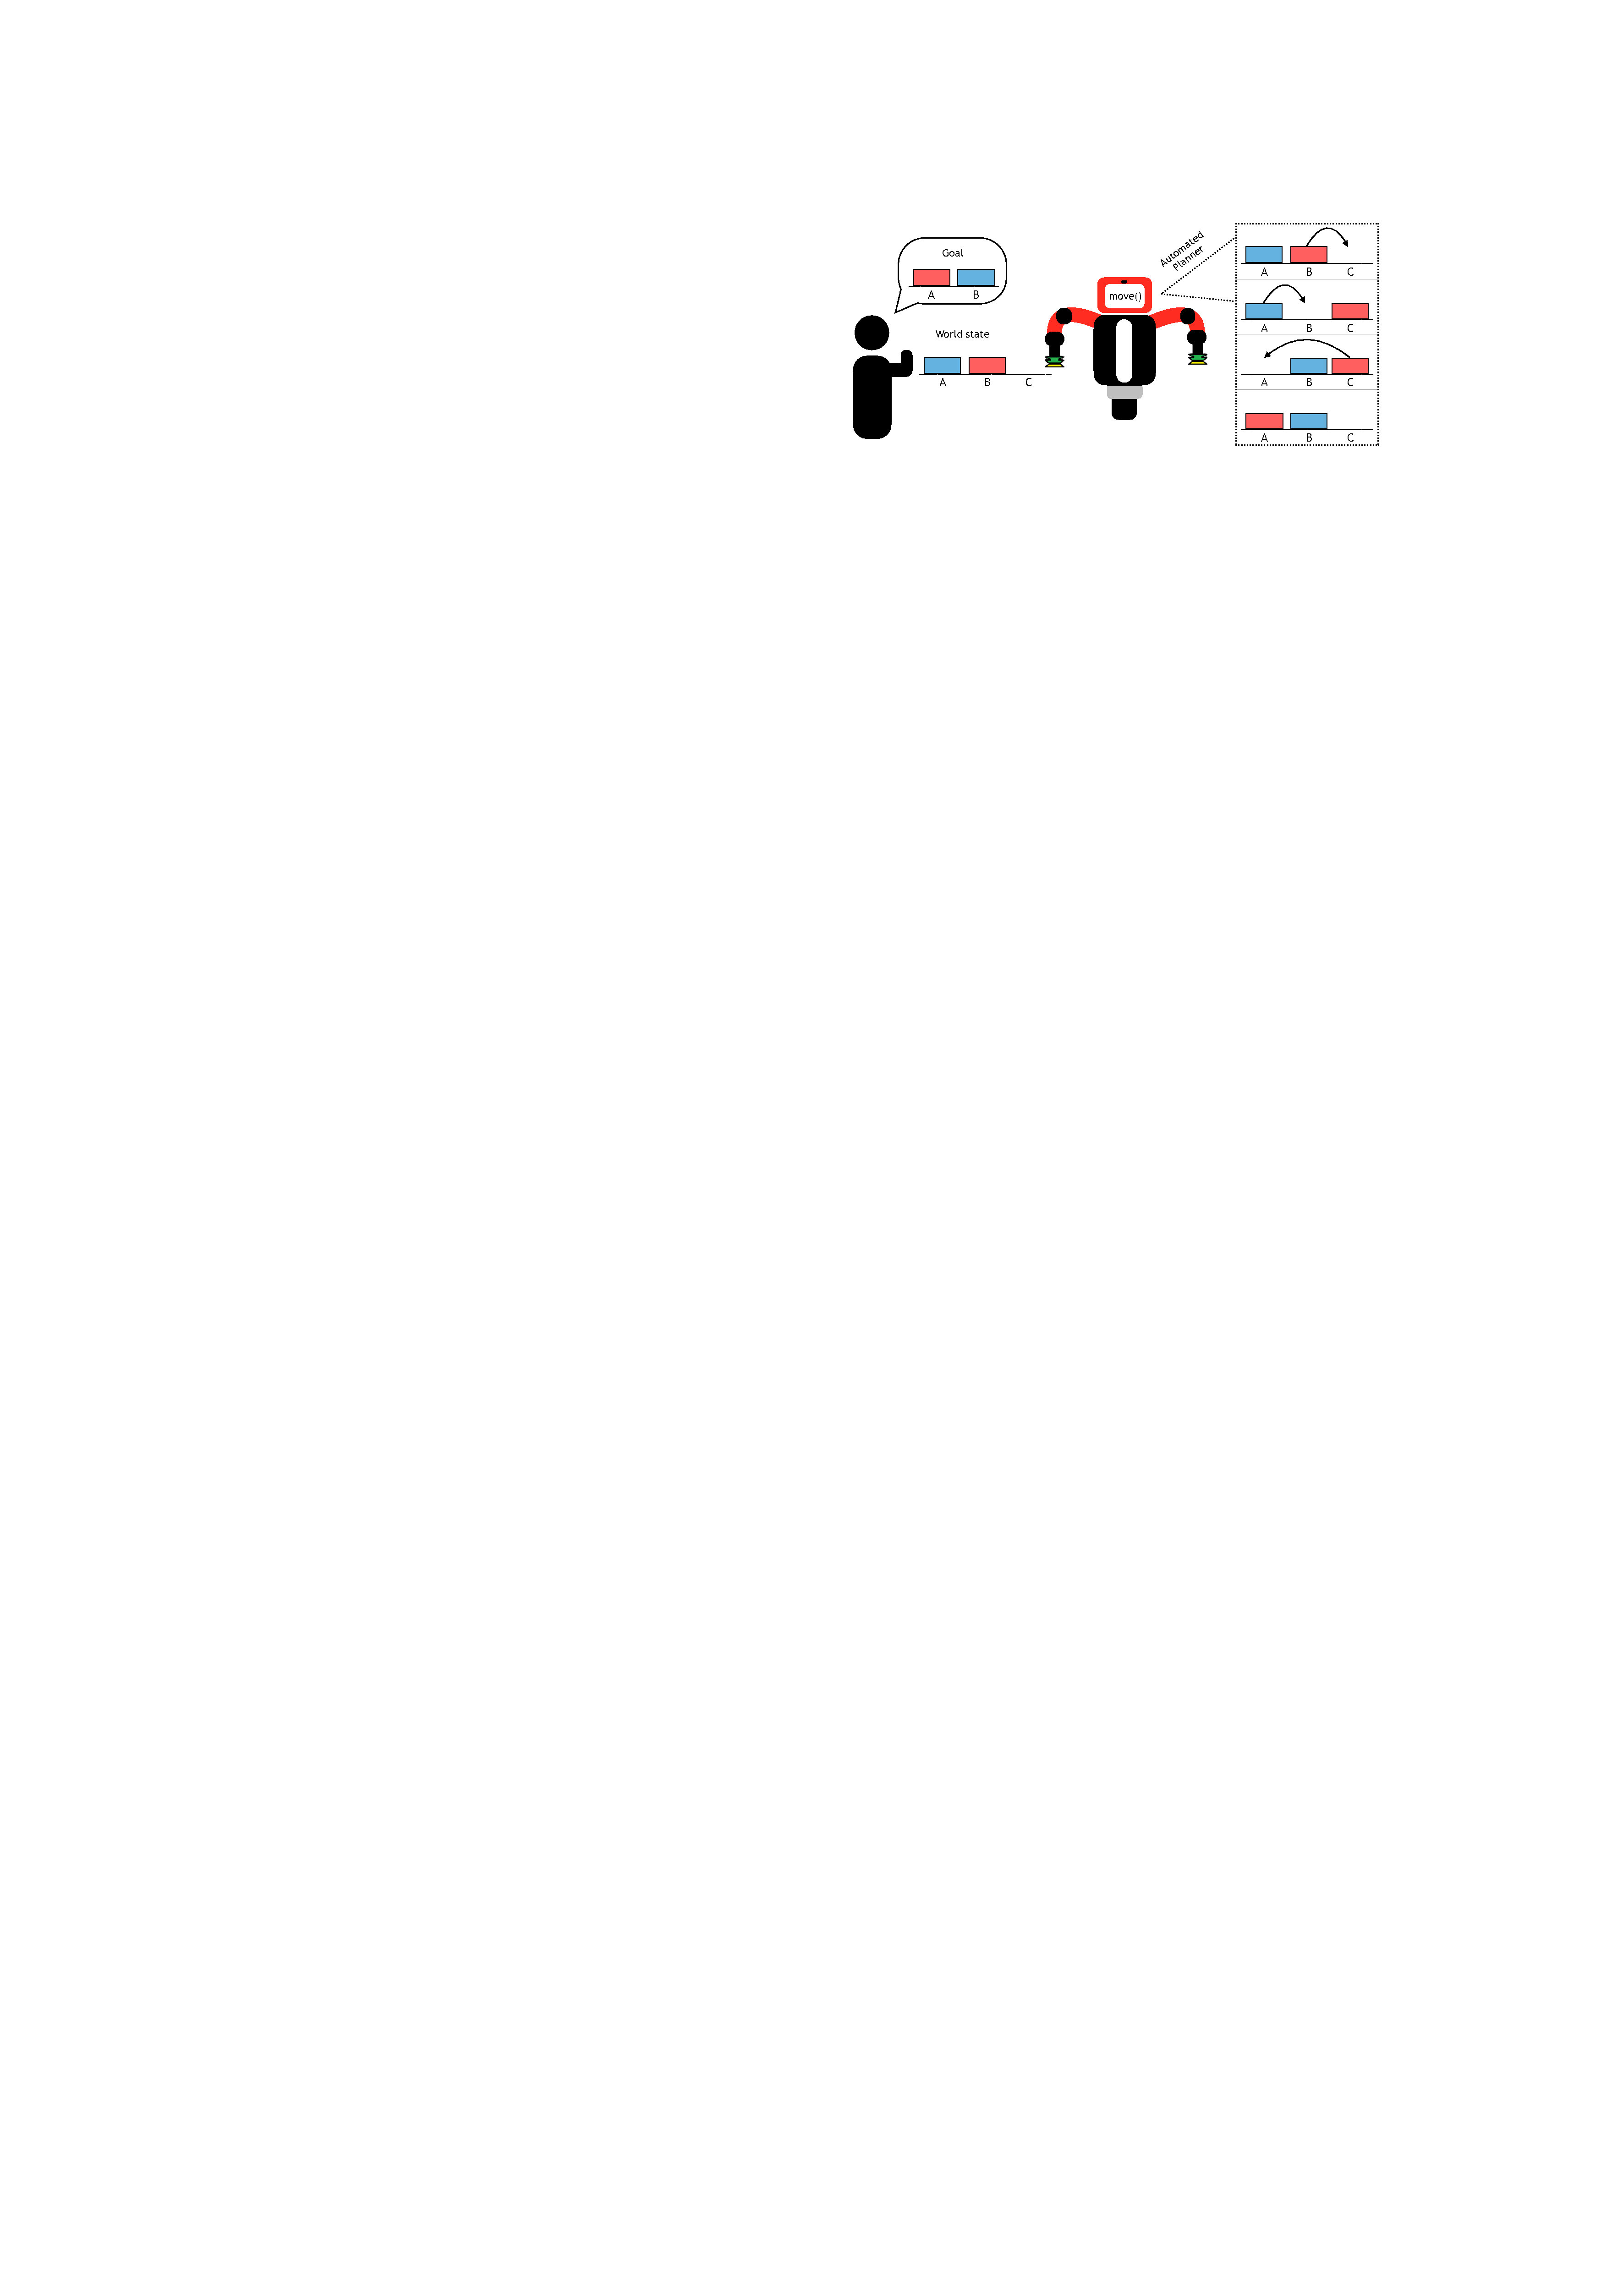
\includegraphics[width=\textwidth]{figures/PbD-AutomatedPlanner}
		\caption{A planning problem can be solved if the robot is provided with a description of the world state, possible actions, and a goal state. The planner can generate an action sequence to solve this problem.}
		\label{fig:Planning domain}
	\end{subfigure}
\hfill
	\begin{subfigure}[t]{0.44\textwidth}
		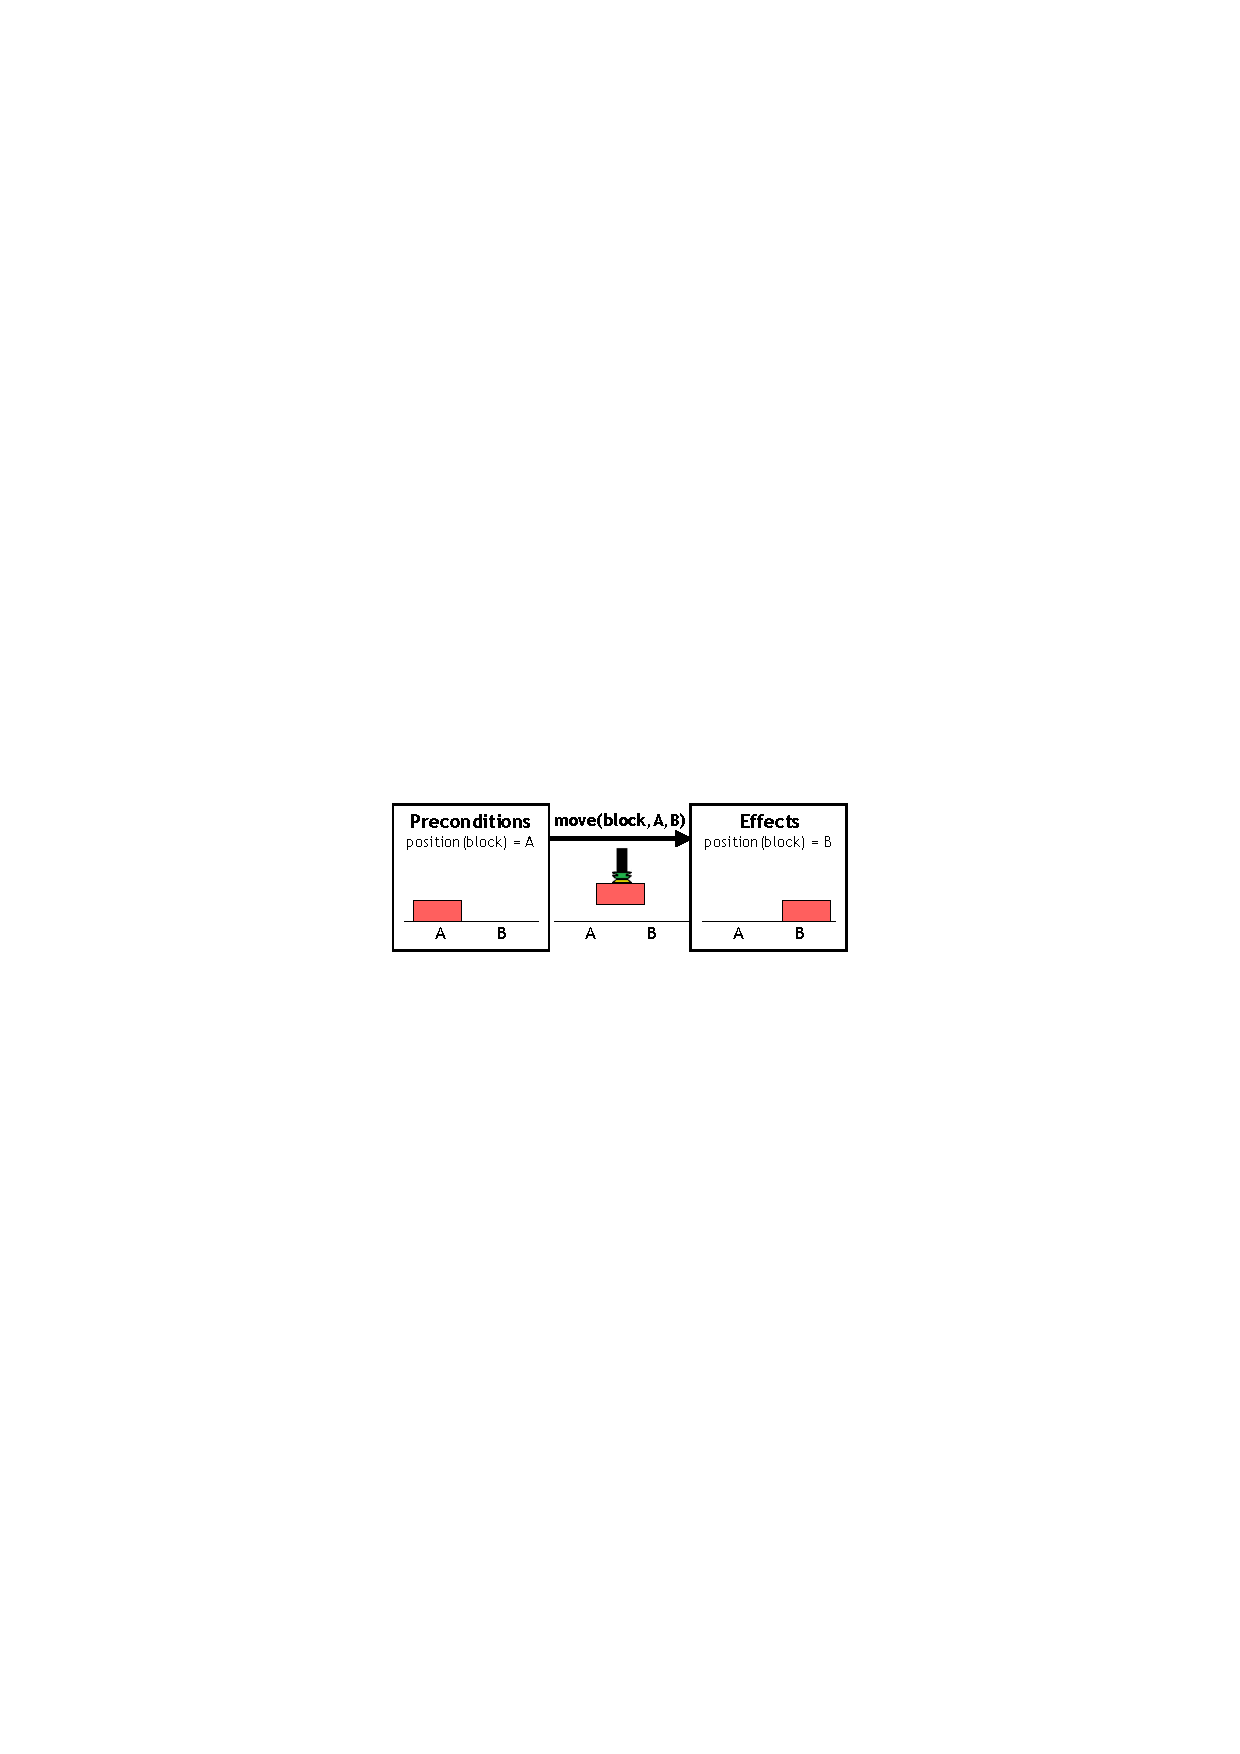
\includegraphics[width=\textwidth]{figures/schema-logic-1}
		\caption{Actions are described in terms of preconditions and effects}
		\label{fig:Planning action}
	\end{subfigure}
	\caption{Illustration of the main Automated Planning concepts}
	\label{fig:Planning domain and action}
\end{figure}
